\documentclass[12pt]{scrartcl}
\usepackage{config}
\usepackage{minted}

%\newcommand\mrh{\color{white}\bfseries}
\newcommand\mrc[1]{\begin{tabular}{@{}l@{}} #1 \end{tabular}}
\setlength\arrayrulewidth{0.8pt}

\usemintedstyle{pastie}

\begin{document}
    \hh{El Flamante Koala}
    
    
    \vspace{10pt}

    
    \hh{Problema}

        Dado un tablero de $K \times K$, donde $K$ es par, y un arreglo $a$ de $N$ parejas de casillas adyacentes en el tablero. Decimos que dos casillas $\{(r_1, c_1), (r_2, c_2)\}$ son adyacentes, si se cumple que $\lvert r_1 - r_2 \lvert + \lvert c_1 - c_2 \lvert = 1$. Un conjunto de parejas de casillas adyacentes es llamado {\itshape Flamante}, si es posible cortar el tablero sobre las líneas que definen las casillas en dos piezas conectadas, congruentes entre sí, y cumpliendo con que todas las parejas del conjunto quedan estrictamente en una de las piezas. Hay un Koala que ama los conjuntos Flamantes, y le gustaría saber cuál es el tamaño más grande, de un subconjunto Flamante, de las $N$ parejas que tienes. Ayuda a nuestro Flamante Koala a resolver el problema.
        
    \hh{Detalles de Implementación}

       Debes implementar la función {\itshape Flamante\_Koala()}. Esta función recibe un entero $K$, el tamaño del tablero; un entero $N$, la cantidad de parejas de casillas adyacentes; y cuatro vectores $r1$, $c1$, $r2$ y $c2$,  con $N$ elementos, las coordenadas de las parejas de casillas adyacentes. Esta función debe regresar un entero, el tamaño máximo de un subconjunto Flamante. 
        La función se vería así:

\begin{minted}{c++}
#include <bits/stdc++.h>
using namespace std;

int Flamante_Koala(int K, int N, vector<int> r1, vector<int> c1,
                    vector<int> r2, vector<int> c2) {
    // Implementa esta función.
}
\end{minted}

    El evaluador llamará la función \textbf{múltiples} veces en cada caso de prueba.

    \hh{Ejemplos}
    
        {\itshape Ejemplo 1:}
        \begin{itemize}
            \item El evaluador llama la función 

            \begin{center}
                {\itshape Flamante\_Koala(4, 8, \{1, 2, 3, 4, 1, 2, 2, 4\}, \{2, 2, 2, 2, 4, 1, 2, 1\}, \{1, 2, 3, 4, 2, 3, 3, 4\}, \{3, 3, 3, 3, 4, 1, 2, 2\})}
            \end{center}
            
            \item en este caso, regresar $7$, daría un veredicto de aceptado. Es posible demostrar que el conjunto de todas las parejas no es flamante, pero el conjunto con las parejas $\{a_1, a_2, a_3, a_4, a_5, a_6, a_8\}$ sí, como se muestra en la figura:
            \begin{center}
                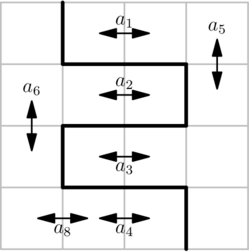
\includegraphics[scale=4]{ej1.png}
            \end{center}
        \end{itemize}
        
        {\itshape Ejemplo 2:}
        \begin{itemize}
            \item El evaluador llama la función 

            \begin{center}
                {\itshape Flamante\_Koala(2, 7, \{1, 2, 1, 1, 1, 1, 1\}, \{1, 1, 1, 1, 2, 1, 2\}, \{1, 2, 1, 2, 2, 2, 2\}, \{2, 2, 2, 1, 2, 1, 2\})}
            \end{center}
            
            \item en este caso, regresar $4$, daría un veredicto de aceptado. 
        \end{itemize}
        
        {\itshape Ejemplo 3:}
        \begin{itemize}
            \item El evaluador llama la función 

            \begin{center}
                {\itshape Flamante\_Koala(6, 1, \{3\}, \{3\}, \{3\}, \{4\})}
            \end{center}
            
            \item en este caso, regresar $1$, daría un veredicto de aceptado. 
        \end{itemize}
        
    \hh{Consideraciones}
        \begin{itemize}
            \item $1 \le N \le 10^5$.
            \item $2 \le K \le 500$. 
            \item $K$ es un número par.
            \item Para todo $0 \le i \le N - 1$, se cumple que $1 \le c1[i], c2[i], r1[i], r2[i] \le K$.
            \item Para todo $0 \le i \le N - 1$, se cumple que las casillas $(c1[i], r1[i])$ y $(c2[i], r2[i])$ son adyacentes.
            \item Sea $S_N$ la suma de los valores de $N$ sobre todas las llamadas de la función en un caso. Se garantiza que $S_N \le 10^5$.
            \item Sea $S_K$ la suma de los valores de $K$ sobre todas las llamadas de la función en un caso. Se garantiza que $S_K \le 500$.
        \end{itemize}
    
    \hh{Subtareas}


    \begin{itemize}
        \item (10 puntos) Para todo $0 \le i \le N - 1$, se cumple que $r1[i] = r2[i]$.
        \item (10 puntos) $N, S_N, K, S_K \le 4$.
        \item (20 puntos) $N, S_N, K, S_K \le 16$.
        \item (50 puntos) Sin restricciones adicionales.
    \end{itemize}
\end{document}
